\documentclass[11pt]{beamer}
\setbeamertemplate{navigation symbols}{}
 \setbeamercovered{transparent}
\usepackage{listings}
%\usetheme{Copenhagen}
\usetheme{Singapore}
%\usetheme{Madrid}
%\usetheme{Hannover}
%\usetheme{boxes}
%\usetheme{Boadilla}
\usefonttheme[onlymath]{serif}
\usecolortheme{beaver}
\usepackage{textpos}
\usepackage{fancyvrb}
\usepackage{xcolor}
\usepackage{multicol}
\usepackage{lipsum}
\parskip 1ex

\newcommand\FontAcolumn{\fontsize{6}{7.2}\selectfont}
\newcommand\FontBcolumn{\fontsize{8}{7.2}\selectfont}
\newcommand\FontCcolumn{\fontsize{10}{7.2}\selectfont}
\newcommand\FontDcolumn{\fontsize{11}{7.2}\selectfont}

\definecolor{gray97}{gray}{.97}
\definecolor{gray75}{gray}{.75}
\definecolor{gray75}{gray}{.45}

\lstdefinestyle{Fortran}{language=[90]Fortran}

\newcommand\FortranStyle
{
\lstset{
frame=Ltb,
framerule=0pt,
columns=fullflexible,
aboveskip=0.5cm,
framextopmargin=3pt,
framexbottommargin=3pt,
framexleftmargin=0.4cm,
framesep=0pt,
rulesep=.4pt,
backgroundcolor=\color{gray97},
rulesepcolor=\color{black},
stringstyle=\ttfamily,
showstringspaces=false,
basicstyle=\ttfamily,
commentstyle=\color{green},
keywordstyle=\color{red},
numbers=left,
numbersep=15pt,
numberstyle=\tiny,
numberfirstline=false,
breaklines=true,
 tabsize=2,
 extendedchars=true,
keepspaces,
}
}

\newcommand\FortranStyleA
{
\lstset{
frame=Ltb,
framerule=0pt,
columns=fullflexible,
aboveskip=0.5cm,
framextopmargin=3pt,
framexbottommargin=3pt,
framexleftmargin=0.4cm,
framesep=0pt,
rulesep=.4pt,
backgroundcolor=\color{gray97},
rulesepcolor=\color{black},
stringstyle=\ttfamily,
showstringspaces=false,
basicstyle=\ttfamily,
commentstyle=\color{green},
keywordstyle=\color{red},
numbersep=15pt,
numberstyle=\tiny,
numberfirstline=false,
breaklines=true,
 tabsize=2,
 extendedchars=true,
keepspaces,
}
}

\def\signed #1{{\leavevmode\unskip\nobreak\hfil\penalty50\hskip2em
  \hbox{}\nobreak\hfil(#1)%
  \parfillskip=0pt \finalhyphendemerits=0 \endgraf}}

\newsavebox\mybox
\newenvironment{aquote}[1]
  {\savebox\mybox{#1}\begin{quote}}
  {\signed{\usebox\mybox}\end{quote}}
  
% items enclosed in square brackets are optional; explanation below
\title{An overview of the Fortran programming language}
%\subtitle{Introduction}
\author{Carlos Cruz\\
Jules Kouatchou\\
Bruce Van Aartsen}
\institute{
  NASA GSFC Code 606 (ASTG)\\
  Greenbelt, Maryland 20771\\[1ex]
%  \texttt{carlos.a.cruz@nasa.gov}
}
\date{October 24, 2018}

\begin{document}

% --- Title page ---
\begin{frame}[plain]
  \titlepage
\end{frame}

\logo{%
  
\includegraphics[width=1cm,height=1cm,keepaspectratio]{../../shared/nasa-ball.png}%
  \hspace{\dimexpr\paperwidth-2cm-5pt}%
  
\includegraphics[width=1cm,height=1cm,keepaspectratio]{../../shared/ssai-logo.png}%
}

% --- Slide

\begin{frame}{Who we are?}

\begin{itemize}
    \item Carlos A. Cruz (Computational Scientist)
    \item Jules Kouatchou (Computational Scientist)
    \item Bruce Van Aartsen (Senior Software Engineer)
\end{itemize}

\end{frame}

% --- Slide

\begin{frame}{Agenda}

\begin{columns}[onlytextwidth,t]
    \begin{column}{0.48\textwidth}
        \textbf{Day 1}

    \begin{itemize}
        \item \textcolor{red}{Introduction}
        \item Variables and data types
        \item Conditionals and loops
        \item Array concepts
        \item Subroutines and functions
        \item Modules and interfaces
        \item File IO
    \end{itemize}
  \end{column}
  \begin{column}{0.48\textwidth}
    \textbf{Day 2}

    \begin{itemize}
        \item Derived types and pointers
        \item Introduction to OOP
        \item Information hiding
        \item Inheritance
        \item Polymorphism
        \item Procedure pointers
        \item Interoperability with C
    \end{itemize}
  \end{column}
\end{columns}

\end{frame}

% --- Slide

\begin{frame}{A Brief History of Fortran}

\begin{itemize}
  \item Origins
  \begin{itemize}
  \scriptsize{
  \item Started ca 1954 by John Backus and his team at IBM
  \item Name comes from \textbf{FOR}mula \textbf{TRAN}slation
  \item First language standard in 1967 (Fortran 66)
  }
  \end{itemize}
  
    \begin{figure}[t]
\centering
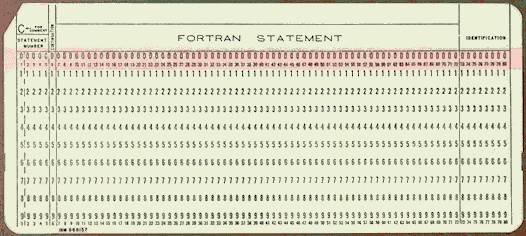
\includegraphics[scale=.3]{fortran-card}
\end{figure}

  \item FORTRAN 77
  \begin{itemize}
  \scriptsize{
  \item New standard to overcome divergence in different implementations (1978)
  }
  \end{itemize}
  
 
\end{itemize}

\end{frame}

% --- Slide

\begin{frame}{A Brief History of Fortran}

 
  
  \parindent0em


\begin{multicols}{2}[\columnsep2em] 


\begin{itemize}
  \item Fortran 90 (All caps were dropped)
  \begin{itemize}
  \scriptsize{
  \item Major revision. Added modules, derived data types, dynamic memory allocation
  \item Retained backward compatibility
  }
  \end{itemize}
  
  \item Fortran 95
  \begin{itemize}
  \scriptsize{
  \item Minor revision. Added several HPC related features; forall, where, pure,
 elemental, pointers
  }
  \end{itemize}
  
    \begin{figure}[t]
\centering
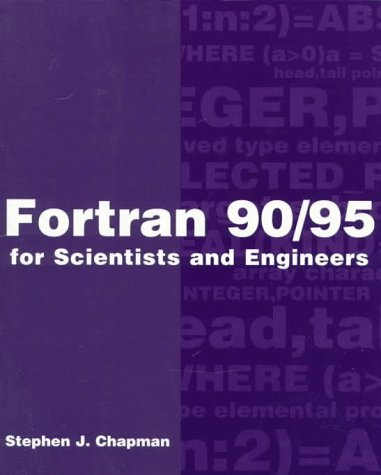
\includegraphics[scale=.3]{Fortran-90-95}
\end{figure}
  
  
\end{itemize}


\columnbreak

\end{multicols}



 
\end{frame}

% --- Slide

\begin{frame}{A Brief History of Fortran}



  \parindent0em


\begin{multicols}{2}[\columnsep2em] 

\begin{itemize}
   
  \item Fortran 2003
  \begin{itemize}
  \scriptsize{
  \item Major revision with many new features including; OO capabilities, procedure pointers, IEEE arithmetic, C interoperability
  }
  \end{itemize}
  
  \item Fortran 2008 (latest \emph{stable} release)
  \begin{itemize}
  \scriptsize{
  \item Minor revision. Added co-arrays and submodules  
  }
  \end{itemize}
  
\end{itemize}

  
    \begin{figure}[t]
\centering
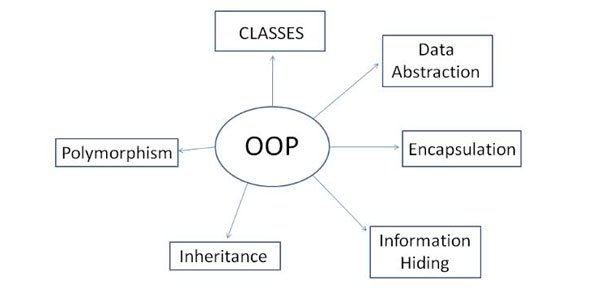
\includegraphics[scale=.25]{oop.jpg}
\end{figure}
  
  


\columnbreak

\end{multicols}




\end{frame}



% --- Slide

\begin{frame}{Why Fortran?}
% https://arstechnica.com/science/2014/05/scientific-computings-future-can-any-coding-language-top-a-1950s-behemoth/

\begin{itemize}
\item Legacy code
\item Expressiveness / ease
 \begin{itemize}
 \item Arrays lie at the heart of all physics/engineering calculations
 \item Little to worry about pointers and memory allocation
 \begin{itemize}
 \item Variables are usually passed by reference, not by value
 \end{itemize}
 \end{itemize}
\item Math support
\item Performance\footnote{Originally proposed as a practical alternative to \textbf{Assembly} language, i.e. it was designed to compete on performance with hand-coded assembler!}
\begin{itemize}
\item Parallelism
\end{itemize}

% \item It's been \textbf{modernized}
 \end{itemize}

\end{frame}


% --- Slide ---

\begin{frame}[fragile]
\frametitle{Fortran is a compiled language}

What is a compiler?
\vfill
A compiler is a \textbf{program} that translates source code written in some high-level language into low-level machine code. The machine code is generally specific to the computer architecture where it was compiled.

% refers to the processing of source code files
%and the creation of an 'object' file
%produces the machine language instructions that correspond to the source code file

\end{frame}

% --- Slide ---

\begin{frame}{Compiler}

What does it do?

\begin{figure}[t]
\centering
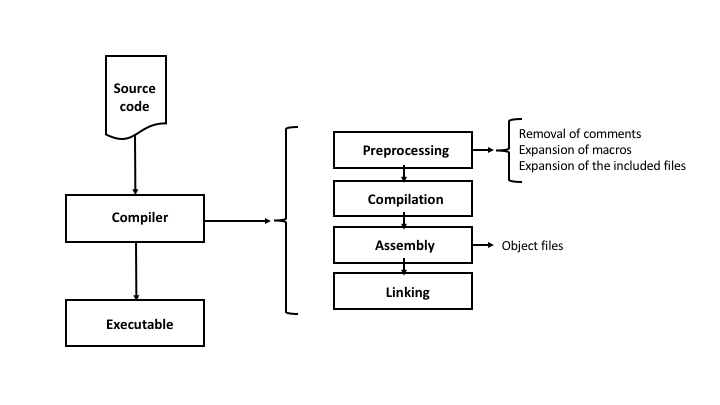
\includegraphics[scale=.3]{compiler}
\end{figure}


\end{frame}

% --- Slide

\begin{frame}{Compilation and Linking}

\begin{itemize}
\item Compilation refers to the processing of source code files and the creation of an 'object' file
which contains the machine language instructions that correspond to the source code file.
\begin{itemize}
\item Compiler errors are usually syntactic in nature.
 \end{itemize}

\item Linking refers to the creation of a single executable file from one or multiple object files
\begin{itemize}
\item Linking errors usually have to do with missing or multiple definitions.
 \end{itemize}

 \end{itemize}

\end{frame}

% --- Slide

\begin{frame}{The GNU Fortran compiler}

The GNU Fortran compiler supports the Fortran 77, 90 and 95 standards completely, parts
of the Fortran 2003 and Fortran 2008 standards, and several vendor extensions. \\
The GNU Fortran compiler has several components:
\begin{itemize}
\item A version of the \emph{gcc} command that also understands and accepts Fortran source code.
\item The \emph{gfortran} command. The difference with \emph{gcc} is that \emph{gfortran} will automatically link the correct libraries to your program.
\item A collection of run-time libraries. 
\item The Fortran compiler itself, \emph{f951}. \emph{f951} \textbf{translates} the source code to assembler code.
 \end{itemize}
GNU Fortran is a part of GCC, the \emph{GNU Compiler Collection}.

\end{frame}


% --- Slide

\begin{frame}[fragile]
\frametitle{Hello World!}

\FortranStyle

 \begin{lstlisting}[style=Fortran]
program hello
print *,'Hello World!'
end program
\end{lstlisting}

\end{frame}


\begin{frame}{Using the compiler}

\begin{itemize}
\item gfortran hello.F90
\begin{itemize}
\item ./a.out
\end{itemize}

 \item gfortran -c hello.F90
\begin{itemize}
\item hello.o
\end{itemize}

\item gfortran -c hello.F90 -o hello.o
\begin{itemize}
\item hello.o
\end{itemize}

\item gfortran -o hello.exe hello.F90
\begin{itemize}
\item ./hello.exe
\end{itemize}

\end{itemize}

\end{frame}

% --- Slide ---

\begin{frame}[fragile]
\frametitle{Linking libraries}

\begin{itemize}
\item Static and dynamic linking
\begin{itemize}
\item Static - performed by linker
\item Dynamic - performed by OS
\end{itemize}
\end{itemize}

\end{frame}

% --- Slide ---

\begin{frame}[fragile]
\frametitle{Libraries}

After compilation we can create a static library using�?ar?�(stands for archiver) 
\begin{Verbatim}
$ gfortran -c *.F90
$ ar r libmystatlib.a *.o
\end{Verbatim}
Or create a dynamic library...
\begin{Verbatim}
$ gfortran -c -fPIC *.F90
$ gfortran -shared -o libmydynlib.so *.o
\end{Verbatim}

\end{frame}


% --- Slide ---

\begin{frame}[fragile]
\frametitle{Make}
What is "make"?
\begin{itemize}
\item The make utility is a tool for managing and maintaining computer programs. It is generally used to build executable programs, libraries, and other files.
\item Created at Bell Labs ca. 1977 
\item The input to make is a file called the makefile
\item makefile  describes a set of targets, which are the objects that can be made.
\end{itemize}
Reference: \url{http://www.gnu.org/software/make/}

\end{frame}



% --- Slide ---

\begin{frame}[fragile]
\frametitle{The makefile}
\begin{itemize}
\item Standard names: GNUmakefile, makefile, Makefile.
\item To run make: "make" or "make <target(s)>"
\item make ?f nonStandardName
\end{itemize}

\end{frame}


% --- Slide ---

\begin{frame}[fragile]
\frametitle{The makefile}

\begin{verbatim}
myfile=a_file.pdf
# This Makefile converts a PS file to a PDF file
include Makefile.local 
sinclude Rules.mk
$(myfile): a_file.ps
          ps2pdf $<
\end{verbatim}

\end{frame}


% --- Slide ---

\begin{frame}[fragile]
\frametitle{The makefile}

\begin{Verbatim}[commandchars=\\\{\}]
\textcolor{red}{myfile=a\_file.pdf}
# This Makefile converts a PS file to a PDF file
include Makefile.local 
sinclude Rules.mk
$(myfile): a_file.ps
          ps2pdf $<
\end{Verbatim}

\end{frame}


% --- Slide

\begin{frame}[fragile]
\frametitle{Conclusion}

Fortran continues and will continue to be a dominant language for large scale simulation of physical systems.
\vfill
\begin{aquote}{John Backus}
I don't know what the technical characteristics of
the standard language for scientific and engineering
computation in the year 2000 will be... but I know it
will be called Fortran.
\end{aquote}

\bigskip
References:
\begin{itemize}
\item \url{https://gcc.gnu.org/fortran/}
\item \url{http://fortranwiki.org/fortran/show/HomePage}
\item \url{https://en.wikipedia.org/wiki/Fortran}
\end{itemize}
\end{frame}

\end{document}
